\documentclass{article}
\usepackage{graphicx}
\usepackage{amsmath, amsfonts, amssymb, amsthm}
\usepackage{tikz, pgfplots, tkz-euclide,calc}
    \usetikzlibrary{patterns,snakes,shapes.arrows}
\usepackage{fancyhdr}
\usepackage{enumerate,enumitem}
\usepackage{cancel}
\usepackage{varwidth}
\usepackage{fontawesome}
\usepackage{derivative}
\usepackage{xfrac}

% TAMBAHKAN PACKAGE SENDIRI KALAU KURANG

\usepackage{geometry}
\geometry{
	total = {160mm, 237mm},
	left = 25mm,
	right = 20mm,
	top = 30mm,
	bottom = 30mm,
}

\pagestyle{fancy}
\fancyhead{}
\fancyfoot{}
\fancyhead[c]{\large{\textbf{Quis 2 jam 9\\Kelas 30}}}
\fancyfoot[r]{\textit{By: Teosofi Hidayah Agung (5002221132)}}
\renewcommand{\headrulewidth}{0pt}
\renewcommand{\footrulewidth}{0pt}

\begin{document}
\pagenumbering{gobble}

    \begin{enumerate}
        \item Roket naik vertikal dan dipantau oleh stasiun radar yang terletak $5$ km dari 
        landasan peluncuran. Berapa cepat roket naik jika tingginya $4$ km dan jaraknya dari 
        stasiun radar bertambah dengan laju $2000$ km/jam?
        \begin{center}
        \begin{tikzpicture}[scale=1.5]
            \coordinate (A) at (0,0);
            \coordinate (B) at (3,0);
            \coordinate (C) at (3,2);

            \draw[dashed] (A)--(C);
            \draw[] (A)--(B);
            \draw[-Latex,blue] ($(B)+(0,0.1)$)--($(C)-(0,0.1)$);
            \draw (B) node[rotate=45] {\faRocket};
            \draw (B) node[below] {\tiny{Roket}};

            \draw (C) node[rotate=45] {\faRocket};

            \draw (A) node[left] {\faFeed};
            \draw (A) node[below right] {\tiny{Stasiun radar}};

            \tkzLabelSegment[above](A,B) {$5$ km};

            \draw[-Latex] (A)--($1/5*(C)$);
        \end{tikzpicture}
        \end{center}

        \textbf{Penyelesaian}:\\~\\
        Ilustrasi gambar:\\
        \begin{tikzpicture}[scale=1.5]
            \coordinate (A) at (0,0);
            \coordinate (B) at (3,0);
            \coordinate (C) at (3,2);

            \draw[dashed] (A)--(C);
            \draw[] (A)--(B);
            \draw[-Latex,blue] (B)--($(C)-(0,0.1)$);
            \draw (C) node[rotate=45] {\faRocket};
            \draw (A) node[left] {\faFeed};

            \tkzLabelSegment[below](A,B) {$5$ km};
            \tkzLabelSegment[right](B,C) {$h$ km};
            \tkzLabelSegment[left](A,C) {\rotatebox{35}{$r$ km}};

            \draw[-Latex] (1,1.3)--(2,2);
            \coordinate[label={[rotate=35]\tiny{$2000$ km/jam}}] (d) at (1.5,1.65);

            \node[rectangle, draw, white, right=1cm, text width=4cm] (eq) at (4,1)
            {\color{black}
            Diketahui:
                \begin{flalign*}
                    h&=4 \textrm{ km}&\\
                    \odv{r}{t}\Big|_{h=4}&=2000 \textrm{ km/jam}&\\
                \end{flalign*}
                };
        \end{tikzpicture}\\
            
        Dari Ilustrasi diatas didapatkan persamaan
        \begin{flalign*}
            r^2&=5^2+h^2&\\
            r^2&=25+h^2
        \end{flalign*}

        Subtitusi $h$ untuk mendapatkan nilai $r$ ketika $h=4$ km
        \begin{flalign*}
            r^2&=5^2+4^2&\\
            r&=\sqrt{5^2+4^2}&\\
            r&=\sqrt{25+16}&\\
            r&=\sqrt{41}
        \end{flalign*}

        Kemudian turunkan kedua ruas terhadap $t$. Dilanjutkan dengan subtitusi nilai $h,r$ dan $\odv{r}{t}$.
        \begin{flalign*}
            \odv*{(r^2)}{t}&=\odv*{(25+h^2)}{t}&\\
            2r\odv{r}{t}&=2h\odv{h}{t}&\\
            r\odv{r}{t}&=h\odv{h}{t}&\\
            (\sqrt{41})(2000)&=(4)\odv{h}{t}&\\
            \odv{h}{t}&=500\sqrt{41}
        \end{flalign*}
        $\therefore$ kecepatan roket saat ketinggiannya $4$ km adalah $500\sqrt{41}$ km/jam.\\

        \item Tentukan nilai maksimum dan minimum dari
        \[f(x)=\begin{cases}
            2x+1,\quad x\leq1\\
            x^2-6x+8,\quad x>1
        \end{cases}\]

        \fancyhead[c]{}
        Pada $[-1,4]$\\~\\
        \textbf{Penyelesaian}:\\
        $f(x)$ dapat ditulis kembali dengan mengiriskan domainnya pada interval yang telah diberikan. $[-1,1]\cup(1,4]$
        \[f(x)=\begin{cases}
            2x+1,\quad -1\leq x\leq1\\
            x^2-6x+8,\quad 1<x\leq4
        \end{cases}\]
        Sebelum menentukan titik ekstrimnya, perlu ditinjau bahwa $f(x)$ kontinu pada selang $[-1,4]$.
        \begin{itemize}
            \item Untuk $f(x)=2x+1,-1\leq x\leq1$ jelas bahwa fungsi linear merupakan fungsi kontinu
            \item Cek kekontinuan di $x=1$.
            \begin{enumerate}[label=\textcircled{\arabic*}]
                \item $f(1)=2(1)+1=3$
                \item $\lim_{x\to 1^-}f(x)=\lim_{x\to 1^-}2x+1=3$\\
                      $\lim_{x\to 1^+}f(x)=\lim_{x\to 1^+}x^2-6x+8=3$\\
                      $\therefore \lim_{x\to 1}f(x)=3$ 
                \item $\lim_{x\to 1}f(x)=f(1)$
                fungsi kontinu di $x=1$
            \end{enumerate}
            \item Untuk $f(x)=x^2-6x+8,1<x\leq4$ jelas bahwa fungsi polinomial merupakan fungsi kontinu. Dapat dicek turunan pertamanya
            \begin{flalign*}
                f'(x)&=2x-6,1<x<4&\\
                &\vbox{
                \halign{#&&\hbox to 1.2in{\cleaders\hbox{#}\hfill}&\hbox to 0pt{\hss$#$\hss}\cr
                & - && $ + $\cr
                $\vert$&-&\vert&-&\vert\cr
                1&&3&&4\cr}
                }\quad\quad\quad\quad \textbf{\textrm{titik kritis di $x=3$}}
            \end{flalign*}
            Titik uji:
            \begin{itemize}[label=$\to$]
                \item $f'(2)=2(2)-6=-2$ \textbf{(Turun)}
                \item $f'(\frac{7}{2})=2(\frac{7}{2})-6=1$ \textbf{(Naik)}
            \end{itemize}
        \end{itemize}

        Step terakhir adalah mencari nilai pada titik-titik ujung dan titik kritis fungsi yang telah dicari
        \begin{center}
            \begin{tabular}{l|cccc}
                $x$&$-1$&$1$&$3$&$4$\\
                \hline
                $f(x)$&$-1$&$3$&$-1$&$0$
            \end{tabular}
        \end{center}
        Setelah itu, bandingkan saja nilai $f(x)$ yang telah didapat.\\

        $\therefore$ nilai maksimumnya adalah $3$ dan nilai minimumnya adalah $-1$.\\
        
        \item Diberikan fungsi $y=4x^3-3x^2+5$
        \begin{enumerate}
            \item Tentukan fungsi naik dan fungsi turun (berikan tanda $f'$)\\
            \textbf{Penyelesaian}: Tentukan turunan pertamanya 
            \begin{flalign*}
                y'&=0&\\
                12x^2-6x&=0&\\
                6x(2x-1)&=0&\\
                x=0\:&\vee\:x=\frac{1}{2}
            \end{flalign*}
            Titik uji:
            \begin{itemize}[label=$\to$]
                \item $f'(-1)=6(-1)(2(-1)-1)=18$ \textbf{(Naik)}
                \item $f'(\frac{1}{4})=6(\frac{1}{4})(2(\frac{1}{4})-1)=-\frac{3}{4}$ \textbf{(Turun)}
                \item $f'(1)=6(1)(2(1)-1)=18$ \textbf{(Naik)}
            \end{itemize}
            \[
            \vbox{\halign{#&&\hbox to 1.2in{\hbox{#}\hfill}&\hbox to 0pt{\hss$#$\hss}\cr
            & \rotatebox[origin=c]{10}{$\quad\quad\xrightarrow{\makebox[2cm]{}}$} && $ \rotatebox[origin=c]{-10}{$\quad\quad\xrightarrow{\makebox[2cm]{}}$} $ && \rotatebox[origin=c]{10}{$\quad\quad\xrightarrow{\makebox[2cm]{}}$} \cr
            \cr
            }
            \halign{#&&\hbox to 1.2in{\cleaders\hbox{#}\hfill}&\hbox to 0pt{\hss$#$\hss}\cr
            & + && $ - $ && + \cr
            \footnotesize{$f'$:}&-&\vert&-&\vert&-&\cr
            &&0&&\frac{1}{2}\cr}
            }
            \]
            \begin{itemize}
                \item Fungsi naik pada $[-\infty,0]$ dan $\left[\frac{1}{2},+\infty\right]$.
                \item Fungsi turun pada $\left[0,\frac{1}{2}\right]$.
            \end{itemize}

            \item Tentukan titik kritis\\
            \textbf{Penyelesaian}: Titik kritis terjadi ketika $x=0\:\vee\:x=\frac{1}{2}$, Sehingga titik kritisnya adalah $(0,5)$ dan $\left(\frac{1}{2},\frac{19}{4}\right)$

            \item Tentukan ekstrim relatif\\
            \textbf{Penyelesaian}: Dengan uji turunan kedua $(y''=24x-6)$ didapatkan
            \begin{itemize}
                \item Untuk $x=0$, maka $y''(0)=-6$. ($f''(x_0)<0$ definisi maksimum relatif)
                \item Untuk $x=0$, maka $y''(\frac{1}{2})=6$. ($f''(x_0)>0$ definisi minimum relatif)
            \end{itemize}
            Atau dapat dilihat dari naik turunnya grafik sebelum dan sesudah titik kritis.\\~\\
            $\therefore$ maksimum relatif ketika $x=0$ dan minimum relatif ketika $x=\frac{1}{2}$. (\textbf{Kedua titik tersebut ekstrim relatif})

            \item Tentukan interval dimana fungsi cekung ke atas dan fungsi cekung ke bawah (berikan tanda $f''$)
            \textbf{Penyelesaian}: Tentukan turunan pertamanya 
            \begin{flalign*}
                y''&=0&\\
                24x-6&=0&\\
                24&=6&\\
                x&=\frac{1}{4}
            \end{flalign*}
            Titik uji:
            \begin{itemize}[label=$\to$]
                \item $f''(0)=24(0)-6=-6$ \textbf{(Cekung ke bawah)}
                \item $f''(1)=24(1)-6=18$ \textbf{(Cekung ke atas)}
            \end{itemize}
            \[
            \vbox{\halign{#&&\hbox to 1.2in{\hbox{#}\hfill}&\hbox to 0pt{\hss$#$\hss}\cr
            & \large{$\quad\quad\quad\quad\bigcap$} && \large{$\quad\quad\quad\quad\bigcup$} \cr
            \cr
            }
            \halign{#&&\hbox to 1.2in{\cleaders\hbox{#}\hfill}&\hbox to 0pt{\hss$#$\hss}\cr
            & - && $ + $\cr
            \footnotesize{$f''$:}&-&\vert&-&\cr
            &&\frac{1}{4}\cr}
            }
            \]
            \begin{itemize}
                \item Fungsi cekung ke atas pada $\left[\frac{1}{4},+\infty\right]$.
                \item Fungsi cekung ke bawah pada $\left[-\infty,\frac{1}{4}\right]$.
            \end{itemize}

            \item Tentukan titik belok\\
            \textbf{Penyelesaian}: Karena arah kecekungan berubah pada $x=\frac{1}{4}$, maka titik beloknya adalah $\left(\frac{1}{4},\frac{39}{8}\right)$.

            \item Sketsalah grafiknya\\
            \begin{tikzpicture}
                \begin{axis}[
                    xmin = -3, xmax = 4, 
                    ymin = -1, ymax = 8,
                    restrict x to domain=-3:8,
                    restrict y to domain=-3:8,
                    axis lines = middle,
                    axis line style={-latex},  
                    xlabel={$x$}, 
                    ylabel={$y$},
                    enlarge x limits={upper={val=0.2}},
                    enlarge y limits=0.05,
                    x label style={at={(ticklabel* cs:1.00)}, inner sep=5pt, anchor=north},
                    y label style={at={(ticklabel* cs:1.00)}, inner sep=2pt, anchor=south east},
                    xtick distance=2, ytick distance=5]

                \addplot [very thick,domain=-5:5, samples=1000, name path=f, color=red]
                {4*x^3 - 3*x^2 + 5};
                
                \draw[fill=blue] (axis cs: 0, 5) circle (0.5mm);
                \draw[fill=blue] (axis cs: {1/2}, {19/4}) circle (0.5mm);
                \draw[dashed] (axis cs: {1/2}, {19/4})--(axis cs: {1/2},0) node [below] {\footnotesize{$\frac{1}{2}$}};
                \draw[dashed] (axis cs: {1/2}, {19/4})--(axis cs: 0,{19/4}) node [below left] {\tiny{$\frac{19}{4}$}};

                \node[color=red, font=\footnotesize] at (axis cs: 3,3) {$f(x)=4x^3 - 3x^2 + 5$};
                \end{axis}
            \end{tikzpicture}\\
        \end{enumerate}

        \item Tangki air berbentuk kerucut dengan jari-jari alasnya $10$ m dan 
        tinggi kerucut $24$ m. Jika air mengalir ke dalam tangki dengan laju 
        $20$ m$^3$/menit, Berapa cepat kedalaman air bertambah pada saat kedalaman
        air $16$ m?
        \begin{center}
        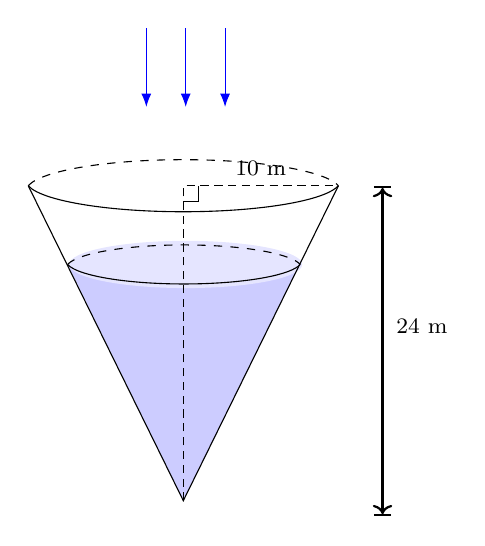
\begin{tikzpicture}
            \draw[dashed] (0,0) arc (170:10:2cm and 0.4cm)coordinate[pos=0] (a);
            \draw (0,0) arc (-170:-10:2cm and 0.4cm)coordinate (b);
            \fill [blue!20!white,opacity=1] (0.5,-1) -- ([yshift=-4cm]$(a)!0.5!(b)$) -- (3.45,-1) -- cycle;
            \fill [blue!10!white,opacity=1,] (2,-1) circle (1.48cm and 0.3cm);
            \draw[densely dashed] ([yshift=-4cm]$(a)!0.5!(b)$) -- node[right,font=\footnotesize] {}coordinate[pos=0.95] (aa)($(a)!0.5!(b)$)
                                    -- node[above,font=\footnotesize] {$10$ m}coordinate[pos=0.1] (bb) (b);
            \draw (aa) -| (bb);
            \draw (a) -- ([yshift=-4cm]$(a)!0.5!(b)$) -- (b);
            \draw[|<->|,thick] (4.5,0)--(4.5,-4.2);
            \coordinate[label=\footnotesize{$24$ m}] () at (5,-2);
            
            \draw[dashed] (0.5,-1) arc (170:10:1.5cm and 0.3cm)coordinate[pos=0] (a');
            \draw (0.5,-1) arc (-170:-10:1.5cm and 0.3cm)coordinate (b');

            \draw [-Latex,blue] (1.5,2) -- (1.5,1);
            \draw [-Latex,blue] (2,2) -- (2,1);
            \draw [-Latex,blue] (2.5,2) -- (2.5,1);
        \end{tikzpicture}
        \end{center}
        \textbf{Penyelesaian}:\\
        Diketahui:
        \[\odv{V}{t}=20\]
        Ditanya:
        \[\odv{h}{t}\Big|_{h=16}=\dots\]\\
        Perhatikan kesebangunan pada segitiga yang terbentuk\\
        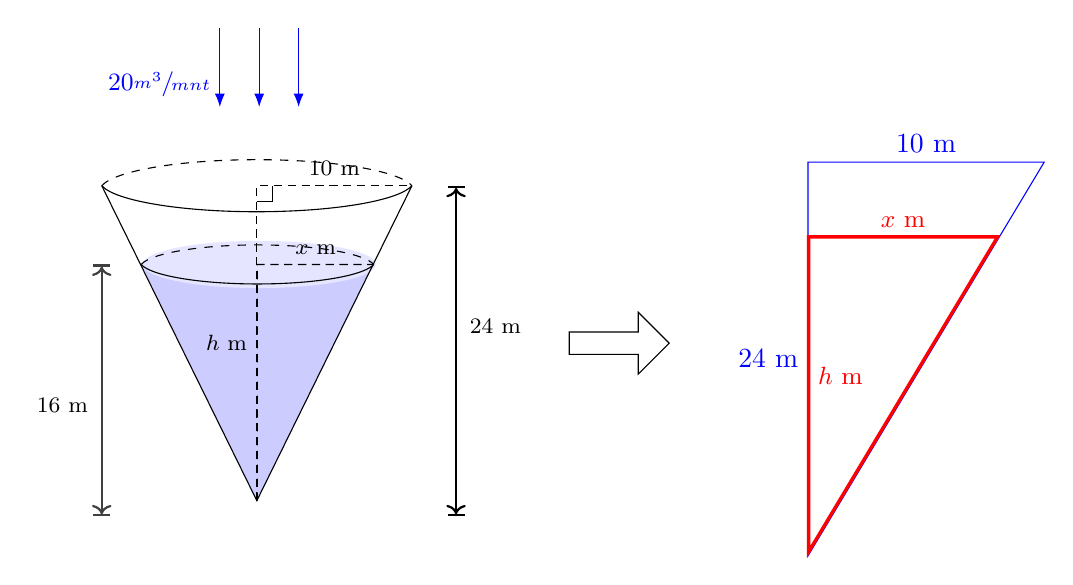
\begin{tikzpicture}
            \draw[dashed] (0,0) arc (170:10:2cm and 0.4cm)coordinate[pos=0] (a);
            \draw (0,0) arc (-170:-10:2cm and 0.4cm)coordinate (b);
            \fill [blue!20!white,opacity=1] (0.5,-1) -- ([yshift=-4cm]$(a)!0.5!(b)$) -- (3.45,-1) -- cycle;
            \fill [blue!10!white,opacity=1,] (2,-1) circle (1.48cm and 0.3cm);
            \draw[densely dashed] ([yshift=-4cm]$(a)!0.5!(b)$) -- node[left,font=\footnotesize] {$h$ m}coordinate[pos=0.95] (aa)($(a)!0.5!(b)$)
                                    -- node[above,font=\footnotesize] {$10$ m}coordinate[pos=0.1] (bb) (b);
            \draw (aa) -| (bb);
            \draw (a) -- ([yshift=-4cm]$(a)!0.5!(b)$) -- (b);
            \draw[|<->|,thick] (4.5,0)--(4.5,-4.2);
            \draw[|<->|,thick,darkgray] (0,-1)--(0,-4.2);
            \coordinate[label=\footnotesize{$24$ m}] () at (5,-2);
            \coordinate[label=\footnotesize{$16$ m}] () at (-0.5,-3);
            
            \draw[dashed] (0.5,-1) arc (170:10:1.5cm and 0.3cm)coordinate[pos=0] (a');
            \draw (0.5,-1) arc (-170:-10:1.5cm and 0.3cm)coordinate (b');
            \draw[densely dashed] ([yshift=-3cm]$(a')!0.5!(b')$) -- coordinate[pos=0.95] (aa')($(a')!0.5!(b')$)
                                    -- node[above,font=\footnotesize] {$x$ m}coordinate[pos=0.1] (bb') (b');

            \draw [-Latex,blue] (1.5,2) -- (1.5,1) node [above left] {\small{$20 \sfrac{m^3}{mnt}$}};
            \draw [-Latex,blue] (2,2) -- (2,1);
            \draw [-Latex,blue] (2.5,2) -- (2.5,1);

            \node[fill=white,single arrow, draw] at (6.5,-2) {\color{white}.........};

            \coordinate (A) at ($(aa)+(10,0.5)$);
            \coordinate (B) at ($(aa)+(7,0.5)$);
            \coordinate (C) at ($(aa)+(7,-4.5)$);
            \draw[blue] (A)--(B)--+(0,-5)--cycle;
            \tkzLabelSegment[above,blue](A,B) {$10$ m};
            \tkzLabelSegment[left,blue](C,B) {$24$ m};

            \coordinate (A') at ($(aa')+(9.4,0.5)$);
            \coordinate (B') at ($(aa')+(7,0.5)$);
            \coordinate (C') at ($(aa)+(7,-3.5)$);
            \draw[red,very thick] (A')--(B')--+(0,-4)--cycle;
            \tkzLabelSegment[above,red](A',B') {\small$x$ m};
            \tkzLabelSegment[below right,red](C',B') {\small $h$ m};
        \end{tikzpicture}
        \begin{flalign*}
            \frac{x}{h}&=\frac{10}{24}&\\
            x&=\frac{5}{12}h
        \end{flalign*}
        Selanjutnya rumuskan volume kerucut 
        \begin{flalign*}
            V&=\frac{1}{3}\pi r^2h&\\
            V&=\frac{1}{3}\pi\left(\frac{5}{12}h\right)^2h\quad\quad\textrm{(\textbf{Subtitusi $x=\frac{5}{12}h$})}&\\
            V&=\frac{1}{3}\pi\left(\frac{25}{144}h^2\right)h&\\
            V&=\frac{25}{432}\pi h^3&\\
        \end{flalign*}
        Turunkan persamaannya terhadap waktu dilanjutkan dengan mensubtitusi nilai-nilai yang diketahui
        \begin{flalign*}
            \odv{V}{t}&=\odv*{\left(\frac{25}{432}\pi h^3\right)}{t}&\\
            \odv{V}{t}&=\frac{25}{432}\pi\odv*{(h^3)}{t}&\\
            \odv{V}{t}&=\frac{25}{432}\pi\cdot3h^2\odv{h}{t}&\\
            \odv{V}{t}&=\frac{25}{144}\pi h^2\odv{h}{t}&\\
            20&=\frac{25}{12^2}\pi(16)^2\odv{h}{t}\quad\quad\textrm{(\textbf{Subtitusi $\odv{V}{t}=20$ dan $h=16$})}&\\
            20&=\frac{25}{\cancelto{3}{12}}\frac{1}{\cancelto{3}{12}}\cdot \cancelto{4}{16}\cdot \cancelto{4}{16}\pi\odv{h}{t}&\\
            20&=\frac{400}{9}\pi\odv{h}{t}&\\
            \odv{h}{t}&=\frac{20}{\frac{400}{9}\pi}&\\
            \odv{h}{t}&=\frac{9}{20\pi}&\\
        \end{flalign*}
        $\therefore$ Kedalaman air bertambah dengan laju $\frac{9}{20\pi}$ m$^3/$menit .
        \newpage
        
    \end{enumerate}
\end{document}